\section{After Partial Pivoting}

\begin{exercise}[3.21, 3.22]
Per i testi degli esercizi consultare il libro di testo.
\end{exercise}
Vedere il codice \nameref{subsection:PALUmethod}.

\begin{exercise}[3.23]
Per il testo dell'esercizio consultare il libro di testo.
\end{exercise}
\begin{itemize}
  \item applicazione al sistema dell'esercizio \ref{exercise:324}: si
osserva che usando il pivoting vengono trovate le soluzioni esatte.
\begin{lstlisting}
octave:25> A
A =
   2.22044604925031e-16   1.00000000000000e+00
   1.00000000000000e+00   0.00000000000000e+00
octave:26> b
b =
   1.00000000000000e+00
   2.50000000000000e-01
octave:27> [L, U, p, unknowns] = PALUmethod(A, b)
L =
   1.00000000000000e+00   0.00000000000000e+00
   2.22044604925031e-16   1.00000000000000e+00
U =
   1.00000000000000e+00   0.00000000000000e+00
   0.00000000000000e+00   1.00000000000000e+00
p =
   2.00000000000000e+00   1.00000000000000e+00
unknowns =
   2.50000000000000e-01
   1.00000000000000e+00
\end{lstlisting}

\item applicazione al primo sistema dell'esercizio \ref{exercise:324}:
\begin{lstlisting}
octave:42> A = [ 
1 0 0 0 0 0 0 0 0 0; 
100 1 0 0 0 0 0 0 0 0; 
0 100 1 0 0 0 0 0 0 0; 
0 0 100 1 0 0 0 0 0 0; 
0 0 0 100 1 0 0 0 0 0; 
0 0 0 0 100 1 0 0 0 0; 
0 0 0 0 0 100 1 0 0 0; 
0 0 0 0 0 0 100 1 0 0; 
0 0 0 0 0 0 0 100 1 0; 
0 0 0 0 0 0 0 0 100 1];
octave:43> x = [1 101*ones(1,9)]';
octave:45> [L, U, p, unknowns] = PALUmethod(A, x);
octave:46> format
octave:47> p
p =
    2    3    4    5    6    7    8    9   10    1
octave:50> format long e
octave:51> unknowns'
ans =
 Columns 1 through 4:
   1.00000000000000e+00   1.00000000000000e+00   9.99999999999925e-01   1.00000000000755e+00
 Columns 5 through 8:
   9.99999999245411e-01   1.00000007545890e+00   9.99992454110141e-01   1.00075458898588e+00
 Columns 9 and 10:
   9.24541101412386e-01   8.54588985876136e+00
\end{lstlisting}

\item applicazione al secondo sistema dell'esercizio \ref{exercise:324}:
\begin{lstlisting}
octave:42> A = [ 
1 0 0 0 0 0 0 0 0 0; 
100 1 0 0 0 0 0 0 0 0; 
0 100 1 0 0 0 0 0 0 0; 
0 0 100 1 0 0 0 0 0 0; 
0 0 0 100 1 0 0 0 0 0; 
0 0 0 0 100 1 0 0 0 0; 
0 0 0 0 0 100 1 0 0 0; 
0 0 0 0 0 0 100 1 0 0; 
0 0 0 0 0 0 0 100 1 0; 
0 0 0 0 0 0 0 0 100 1];
octave:43> x = [1 101*ones(1,9)]';
octave:54> y = .1*x;
octave:55> [L, U, p, unknowns] = PALUmethod(A, y);
octave:56> format
octave:57> p
p =
    2    3    4    5    6    7    8    9   10    1
octave:58> format long e
octave:59> unknowns'
ans =
 Columns 1 through 4:
   1.00000000000000e-01   1.00000000000001e-01   9.99999999998550e-02   1.00000000014504e-01
 Columns 5 through 8:
   9.99999985496383e-02   1.00000145036173e-01   9.99854963826791e-02   1.01450361732092e-01
 Columns 9 and 10:
  -4.50361732092139e-02   1.46036173209214e+01
\end{lstlisting} 
\item applicazione al sistema $B\vect{x} = \vect{f}$:
\begin{lstlisting}
octave:59> format 
octave:60> B = [0 1 1; 1 0 1; 2 3 4]
B =
   0   1   1
   1   0   1
   2   3   4
octave:61> f = [1;0;3];
octave:62> [L, U, p, unknowns] = PALUmethod(B, f);
octave:63> L
L =

   1.00000000000000e+00   0.00000000000000e+00   0.00000000000000e+00
   5.00000000000000e-01   1.00000000000000e+00   0.00000000000000e+00
   0.00000000000000e+00  -6.66666666666667e-01   1.00000000000000e+00

octave:64> U
U =
   2.00000000000000e+00   3.00000000000000e+00   4.00000000000000e+00
   0.00000000000000e+00  -1.50000000000000e+00  -1.00000000000000e+00
   0.00000000000000e+00   0.00000000000000e+00   3.33333333333333e-01
octave:66> p
p =
   3   2   1
octave:67> format long e
octave:68> unknowns 
unknowns =
   0.00000000000000e+00
   1.00000000000000e+00
   0.00000000000000e+00
octave:72> B*unknowns - f
ans =
   0
   0
   0
\end{lstlisting}
\end{itemize}

\begin{exercise}[3.24]
\label{exercise:324}
Per il testo dell'esercizio consultare il libro di testo.
\end{exercise}
\begin{lstlisting}
octave:8> A = [eps 1; 1 0], b = [1; 1/4]
A =
   2.22044604925031e-16   1.00000000000000e+00
   1.00000000000000e+00   0.00000000000000e+00
b =
   1.00000000000000e+00
   2.50000000000000e-01
octave:9> A\b
ans =
   2.50000000000000e-01
   1.00000000000000e+00
octave:10> L = [1 0; 1/eps 1], U = [eps 1; 0 -1/eps]
L =
   1.00000000000000e+00   0.00000000000000e+00
   4.50359962737050e+15   1.00000000000000e+00
U =
   2.22044604925031e-16   1.00000000000000e+00
   0.00000000000000e+00  -4.50359962737050e+15
octave:11> (L*U) - A
ans =
   0.00000000000000e+00   0.00000000000000e+00
   0.00000000000000e+00   0.00000000000000e+00
octave:12> U\(L\b)
ans =
   0.00000000000000e+00
   1.00000000000000e+00
\end{lstlisting}
La riga \emph{octave:9} restituisce la soluzione esatta del sistema, ovvero il
vettore $\vect{x} = \bigl [ \begin{smallmatrix}
.25 \\
1
\end{smallmatrix}\bigr ]$.

La riga \emph{octave:11} dimostra che $A = LU$ quindi $0 = LU - A$, le matrici
di fattorizzazione sono corrette.

La riga \emph{octave:12} dimostra che il metodo di fattorizzazione $LU$ senza
pivoting risulta essere mal condizionato, infatti la prima componente
$\tilde{x}_{1} = 0 \not = .25 = x_{1}$.

\begin{exercise}[3.25]
Per il testo dell'esercizio consultare il libro di testo.
\end{exercise}
Per calcolare $k_{\infty}(A)$ \`e necessario calcolare l'inversa:
\begin{displaymath}
\begin{bmatrix}
1 \\
-100 & 1 \\ 
100^{2} & -100 & 1\\ 
-100^{4} & 100^{2} & -100 & 1\\
\vdots & & & & \ddots \\
-100^{16} & 100^{14} & -100^{12} & \cdots & \cdots &  1
\end{bmatrix} = A^{-1}
\end{displaymath}
Questo l'output del codice:
\begin{lstlisting}
octave:35> cond(A,Inf)
warning: inverse: matrix singular to machine precision, rcond = 9.80198e-21
ans =  1.0202e+20
\end{lstlisting}

\begin{exercise}[3.26]
\label{exercise:326}
Per il testo dell'esercizio consultare il libro di testo.
\end{exercise}
Questo il codice che verifica che i vettori $\vect{x}, \vect{y}$ sono soluzioni
rispettivamente delle equazioni $A\vect{x} = \vect{b}, A\vect{y} = \vect{c}$:
\begin{lstlisting}
octave:41> A
A =

     1     0     0     0     0     0     0     0     0     0
   100     1     0     0     0     0     0     0     0     0
     0   100     1     0     0     0     0     0     0     0
     0     0   100     1     0     0     0     0     0     0
     0     0     0   100     1     0     0     0     0     0
     0     0     0     0   100     1     0     0     0     0
     0     0     0     0     0   100     1     0     0     0
     0     0     0     0     0     0   100     1     0     0
     0     0     0     0     0     0     0   100     1     0
     0     0     0     0     0     0     0     0   100     1

octave:42> b = [1;101;101;101;101;101;101;101;101;101];
octave:43> x = [1;1;1;1;1;1;1;1;1;1];
octave:44> A*x - b
ans =
   0
   0
   0
   0
   0
   0
   0
   0
   0
   0
octave:45> c = .1*b;
octave:46> y = [.1;.1;.1;.1;.1;.1;.1;.1;.1;.1];
octave:47> A*y - c
ans =
   0
   0
   0
   0
   0
   0
   0
   0
   0
   0
\end{lstlisting}
Implemento le istruzioni:
\begin{lstlisting}
octave:50> b = [1 101*ones(1,9)]';
octave:51> x(1) = b(1);
octave:52> for i=2:10, x(i) = b(i) - 100*x(i-1); end
octave:53> x = x(:)
x =
   1
   1
   1
   1
   1
   1
   1
   1
   1
   1
octave:54> c = .1*[1 101*ones(1,9)]';
octave:55> y(1) = c(1);
octave:56> for i=2:10, y(i) = c(i) - 100*y(i-1); end
octave:57> y = y(:)
y =
    0.100000
    0.100000
    0.100000
    0.100000
    0.100000
    0.100000
    0.099986
    0.101407
   -0.040702
   14.170153
octave:62> (y-yexact) ./ yexact  
ans =
     0.00000
     0.00000
    -0.00000
     0.00000
    -0.00000
     0.00000
    -0.00014
     0.01407
    -1.40702
   140.70153
\end{lstlisting}
Si osserva che il vettore $\vect{y}$, soluzione esatta del secondo sistema, non
\`e uguale al vettore approssimato dal secondo set di istruzioni: il comando
\emph{octave:62} calcola il vettore degli errori relativi che si commettono e si
nota che per l'ultima componente si ha un errore molto significativo. Questo \`e
dovuto dal fatto che le componenti del vettore dei termini noti $\vect{c}$ non
\`e possibile rappresentarle correttamente in macchina (0.1 ha rappresentazione
infinita periodica in binario). Questi errori di rappresentazione si sommano
nelle 9 iterazioni che vengono fatte dal ciclo for, risultando significative per
la decima componente.

\begin{exercise}[3.28]
Per il testo dell'esercizio consultare il libro di testo.
\end{exercise}
\begin{proof}
Si vuole dimostrare:
\begin{displaymath}
\beta = -\frac{v_{1}}{\alpha} = \frac{2}{\hat{\vect{v}}^{T}\hat{\vect{v}}},
\quad
\text{con} \quad \hat{\vect{v}} = \frac{\vect{v}}{v_{1}}
\end{displaymath} 
\begin{itemize}
  \item Verifico la concordanza dei segni:
  \begin{displaymath}
    \frac{2}{\hat{\vect{v}}^{T}\hat{\vect{v}}} > 0
  \end{displaymath}
  $\hat{\vect{v}}^{T}\hat{\vect{v}} > 0$ per definizione di norma euclidea.
  Deve quindi valere:
  \begin{displaymath}
  \frac{v_{1}}{\alpha} < 0
  \end{displaymath}
  posso sostituire $v_{1} = z_{1} - \alpha$ e $\alpha =
  -sign(z_{1})||\vect{z}||_{2}$ e $sign(a) = \left \{ \begin{array}{ll} 1 & if
  \quad a \geq 0 \\ -1 & if \quad a
  < 0 \end{array} \right .$ ottenendo:
  \begin{displaymath}
  \frac{z_{1}}{\alpha} - 1 < 0 \Rightarrow \frac{z_{1}}{\alpha} < 1 \Rightarrow
  \frac{sign(z_{1})|z_{1}|}{-sign(z_{1})||\vect{z}||_{2}} < 1 \Rightarrow
  \frac{|z_{1}|}{||\vect{z}||_{2}} > -1
  \end{displaymath}
  Ma questo \`e vero in quanto $|z_{1}| > 0$ per definizione di $|\cdot|$ e
  $||\vect{z}||_{2} > 0$ per definizione di norma euclidea, quindi
  $\frac{|z_{1}|}{||\vect{z}||_{2}} > 0 > -1$. I segni concordano.
  
  \item dimostro l'uguaglianza dei due membri:
  
  Per il primo membro vale:
  \begin{displaymath}
  	-\frac{v_{1}}{\alpha} = 
  	- \frac{sign(z_{1})|z_{1}| -
  	(-sign(z_{1})||\vect{z}||_{2})}{-sign(z_{1})||\vect{z}||_{2}} = -
  	\frac{sign(z_{1})(|z_{1}| + ||\vect{z}||_{2})}{-sign(z_{1})||\vect{z}||_{2}}
  	= \frac{|z_{1}| + ||\vect{z}||_{2}}{||\vect{z}||_{2}}
  \end{displaymath} 
  Per il secondo membro vale:
  \begin{displaymath}
  \begin{split}   
  	\hat{\vect{v}}^{T}\hat{\vect{v}} &= \frac{\vect{v}^{T}\vect{v}}{v_{1}^{2}} =
  	\frac{(\vect{z}^{T} - \alpha \vect{e}_{i}^{T})(\vect{z} -\alpha
  	\vect{e}_{i})}{v_{1}^{2}} = 
  	\frac{\vect{z}^{T}\vect{z} -\alpha \vect{z}^{T}\vect{e}_{i} - \alpha
  	\vect{e}_{i}^{T}\vect{z}
  	+\alpha^{2}\vect{e}_{i}^{T}\vect{e}_{i}}{v_{1}^{2}} = \\
  	&= \frac{\alpha^{2} -\alpha z_{1} - \alpha
  	z_{1}+\alpha^{2}}{v_{1}^{2}} = \frac{2||\vect{z}||_{2}^{2} -2\alpha
  	z_{1}}{v_{1}^{2}} = \frac{2||\vect{z}||_{2}^{2}
  	-2(-sign(z_{1})||\vect{z}||_{2} sign(z_{1})|z_{1}|)}{v_{1}^{2}} = \\
  	&= \frac{2||\vect{z}||_{2}^{2}
  	+2||\vect{z}||_{2}|z_{1}|}{v_{1}^{2}} =
  	\frac{2||\vect{z}||_{2}(||\vect{z}||_{2} +|z_{1}|)}{v_{1}^{2}}
  \end{split}
  \end{displaymath}
  Ma vale che $v_{1} = z_{1} - \alpha = sign(z_{1}) -
  (-sign(z_{1})||\vect{z}||_{2}) = sign(z_{1})(|z_{1}| + ||\vect{z}||_{2})$, per
  cui vale \\$v_{1}^{2} = (|z_{1}| + ||\vect{z}||_{2})^{2}$, quindi posso
  sostituire e semplificare ottenendo:
  \begin{displaymath}
  	\hat{\vect{v}}^{T}\hat{\vect{v}} = \frac{2||\vect{z}||_{2}}{||\vect{z}||_{2}+|z_{1}|}
  \end{displaymath}
  Posso invertire potendo riscrivere il secondo membro come:
  \begin{displaymath}
  \frac{2}{\hat{\vect{v}}^{T}\hat{\vect{v}}} =
  \frac{||\vect{z}||_{2}+|z_{1}|}{||\vect{z}||_{2}} = -\frac{v_{1}}{\alpha} = \beta 
  \end{displaymath}
  e questo termina la prova.
\end{itemize}
\end{proof}

\begin{exercise}[3.29, 3.30]
Per i testi degli esercizi consultare il libro di testo.
\end{exercise}
Vedere il codice \nameref{subsection:QRmethod}.

\begin{exercise}[3.31]
Per il testo dell'esercizio consultare il libro di testo.
\end{exercise}
Questa l'implementazione:
\begin{lstlisting}
octave:37> A = [3 2 1; 1 2 3; 1 2 1; 2 1 2]
A =
   3   2   1
   1   2   3
   1   2   1
   2   1   2
octave:38> b = [10*ones(1,4)]'
b =
   10
   10
   10
   10
octave:39> [houseHolderVectors, Rhat, R, Q, g1, g2, unknowns, residue] =
QRmethod(A,b) houseHolderVectors =
   1.00000   0.00000   0.00000
   0.14550   1.00000   0.00000
   0.14550   0.40559   1.00000
   0.29099  -0.15589  -0.47436
Rhat =
  -3.87298  -3.09839  -2.84019
   0.00000  -1.84391  -1.73544
   0.00000   0.00000   1.98030
   0.00000   0.00000   0.00000
R =
  -3.87298  -3.09839  -2.84019
   0.00000  -1.84391  -1.73544
   0.00000   0.00000   1.98030
Q =
  -0.77460   0.21693  -0.41586  -0.42426
  -0.25820  -0.65079   0.57429  -0.42426
  -0.25820  -0.65079  -0.43566   0.56569
  -0.51640   0.32540   0.55448   0.56569
g1 =
  -18.0739
   -7.5926
    2.7724
g2 =  2.8284
unknowns =
   1.4000
   2.8000
   1.4000
residue =
   1.2000
   1.2000
  -1.6000
  -1.6000
octave:40> R*unknowns -g1 
ans =
   0.0000e+00
  -8.8818e-16
   0.0000e+00
octave:41> norm(R*unknowns -g1 )^2 + norm(g2 )^2
ans =  8.0000
octave:42> r = Q*Rhat*unknowns - b
r =
   1.2000
   1.2000
  -1.6000
  -1.6000
octave:43> norm(r)^2
ans =  8.0000
octave:44> Q*Rhat
ans =
   3.00000   2.00000   1.00000
   1.00000   2.00000   3.00000
   1.00000   2.00000   1.00000
   2.00000   1.00000   2.00000
octave:45> r/norm(r)
ans =
   0.42426
   0.42426
  -0.56569
  -0.56569
\end{lstlisting}
 
\begin{exercise}[3.32]
Per il testo dell'esercizio consultare il libro di testo.
\end{exercise}
Implemento lanciando la funzione \nameref{subsection:functionExercise332}: 
\begin{lstlisting}
octave:13> [unknowns, givenUnknowns] = functionExercise332(0)
unknowns =
 Columns 1 through 3:
   9.63228005156231e+00   9.96322800515623e+00   9.98161400257811e+00
   6.83859974218842e+00   5.18385997421884e+00   5.09192998710942e+00
 Columns 4 through 6:
   9.99632280051562e+00   9.99816140025781e+00   9.99963228005156e+00
   5.01838599742188e+00   5.00919299871094e+00   5.00183859974219e+00
 Columns 7 and 8:
   9.99981614002578e+00   9.99996322800516e+00
   5.00091929987110e+00   5.00018385997422e+00

givenUnknowns =
 Columns 1 through 3:
   9.63228005156232e+00   9.96322800515623e+00   9.98161400257811e+00
   6.83859974218843e+00   5.18385997421885e+00   5.09192998710943e+00
 Columns 4 through 6:
   9.99632280051562e+00   9.99816140025781e+00   9.99963228005156e+00
   5.01838599742189e+00   5.00919299871094e+00   5.00183859974219e+00
 Columns 7 and 8:
   9.99981614002578e+00   9.99996322800515e+00
   5.00091929987110e+00   5.00018385997422e+00
\end{lstlisting}
Riporto quattro grafici relativi a quattro diversi valori di $gamma$.
I grafici in blu sono relativi alla soluzione calcolata con l'implementazione
\nameref{subsection:QRmethod}, mentre i grafici verdi (a obiettivo) e rossi sono
invece relativi al codice dato nell'esercizio. 
\\\\
$gamma = 10$:
\begin{center}
% GNUPLOT: LaTeX picture with Postscript
\begingroup
  \makeatletter
  \providecommand\color[2][]{%
    \GenericError{(gnuplot) \space\space\space\@spaces}{%
      Package color not loaded in conjunction with
      terminal option `colourtext'%
    }{See the gnuplot documentation for explanation.%
    }{Either use 'blacktext' in gnuplot or load the package
      color.sty in LaTeX.}%
    \renewcommand\color[2][]{}%
  }%
  \providecommand\includegraphics[2][]{%
    \GenericError{(gnuplot) \space\space\space\@spaces}{%
      Package graphicx or graphics not loaded%
    }{See the gnuplot documentation for explanation.%
    }{The gnuplot epslatex terminal needs graphicx.sty or graphics.sty.}%
    \renewcommand\includegraphics[2][]{}%
  }%
  \providecommand\rotatebox[2]{#2}%
  \@ifundefined{ifGPcolor}{%
    \newif\ifGPcolor
    \GPcolortrue
  }{}%
  \@ifundefined{ifGPblacktext}{%
    \newif\ifGPblacktext
    \GPblacktexttrue
  }{}%
  % define a \g@addto@macro without @ in the name:
  \let\gplgaddtomacro\g@addto@macro
  % define empty templates for all commands taking text:
  \gdef\gplbacktext{}%
  \gdef\gplfronttext{}%
  \makeatother
  \ifGPblacktext
    % no textcolor at all
    \def\colorrgb#1{}%
    \def\colorgray#1{}%
  \else
    % gray or color?
    \ifGPcolor
      \def\colorrgb#1{\color[rgb]{#1}}%
      \def\colorgray#1{\color[gray]{#1}}%
      \expandafter\def\csname LTw\endcsname{\color{white}}%
      \expandafter\def\csname LTb\endcsname{\color{black}}%
      \expandafter\def\csname LTa\endcsname{\color{black}}%
      \expandafter\def\csname LT0\endcsname{\color[rgb]{1,0,0}}%
      \expandafter\def\csname LT1\endcsname{\color[rgb]{0,1,0}}%
      \expandafter\def\csname LT2\endcsname{\color[rgb]{0,0,1}}%
      \expandafter\def\csname LT3\endcsname{\color[rgb]{1,0,1}}%
      \expandafter\def\csname LT4\endcsname{\color[rgb]{0,1,1}}%
      \expandafter\def\csname LT5\endcsname{\color[rgb]{1,1,0}}%
      \expandafter\def\csname LT6\endcsname{\color[rgb]{0,0,0}}%
      \expandafter\def\csname LT7\endcsname{\color[rgb]{1,0.3,0}}%
      \expandafter\def\csname LT8\endcsname{\color[rgb]{0.5,0.5,0.5}}%
    \else
      % gray
      \def\colorrgb#1{\color{black}}%
      \def\colorgray#1{\color[gray]{#1}}%
      \expandafter\def\csname LTw\endcsname{\color{white}}%
      \expandafter\def\csname LTb\endcsname{\color{black}}%
      \expandafter\def\csname LTa\endcsname{\color{black}}%
      \expandafter\def\csname LT0\endcsname{\color{black}}%
      \expandafter\def\csname LT1\endcsname{\color{black}}%
      \expandafter\def\csname LT2\endcsname{\color{black}}%
      \expandafter\def\csname LT3\endcsname{\color{black}}%
      \expandafter\def\csname LT4\endcsname{\color{black}}%
      \expandafter\def\csname LT5\endcsname{\color{black}}%
      \expandafter\def\csname LT6\endcsname{\color{black}}%
      \expandafter\def\csname LT7\endcsname{\color{black}}%
      \expandafter\def\csname LT8\endcsname{\color{black}}%
    \fi
  \fi
  \setlength{\unitlength}{0.0500bp}%
  \begin{picture}(7680.00,5760.00)%
    \gplgaddtomacro\gplbacktext{%
      \colorrgb{0.00,0.00,0.00}%
      \put(866,634){\makebox(0,0)[r]{\strut{}-20}}%
      \colorrgb{0.00,0.00,0.00}%
      \put(866,1304){\makebox(0,0)[r]{\strut{}0}}%
      \colorrgb{0.00,0.00,0.00}%
      \put(866,1975){\makebox(0,0)[r]{\strut{}20}}%
      \colorrgb{0.00,0.00,0.00}%
      \put(866,2645){\makebox(0,0)[r]{\strut{}40}}%
      \colorrgb{0.00,0.00,0.00}%
      \put(866,3316){\makebox(0,0)[r]{\strut{}60}}%
      \colorrgb{0.00,0.00,0.00}%
      \put(866,3986){\makebox(0,0)[r]{\strut{}80}}%
      \colorrgb{0.00,0.00,0.00}%
      \put(866,4657){\makebox(0,0)[r]{\strut{}100}}%
      \colorrgb{0.00,0.00,0.00}%
      \put(866,5327){\makebox(0,0)[r]{\strut{}120}}%
      \colorrgb{0.00,0.00,0.00}%
      \put(1494,414){\makebox(0,0){\strut{}0}}%
      \colorrgb{0.00,0.00,0.00}%
      \put(2486,414){\makebox(0,0){\strut{}2}}%
      \colorrgb{0.00,0.00,0.00}%
      \put(3478,414){\makebox(0,0){\strut{}4}}%
      \colorrgb{0.00,0.00,0.00}%
      \put(4470,414){\makebox(0,0){\strut{}6}}%
      \colorrgb{0.00,0.00,0.00}%
      \put(5462,414){\makebox(0,0){\strut{}8}}%
      \colorrgb{0.00,0.00,0.00}%
      \put(6454,414){\makebox(0,0){\strut{}10}}%
    }%
    \gplgaddtomacro\gplfronttext{%
    }%
    \gplbacktext
    \put(0,0){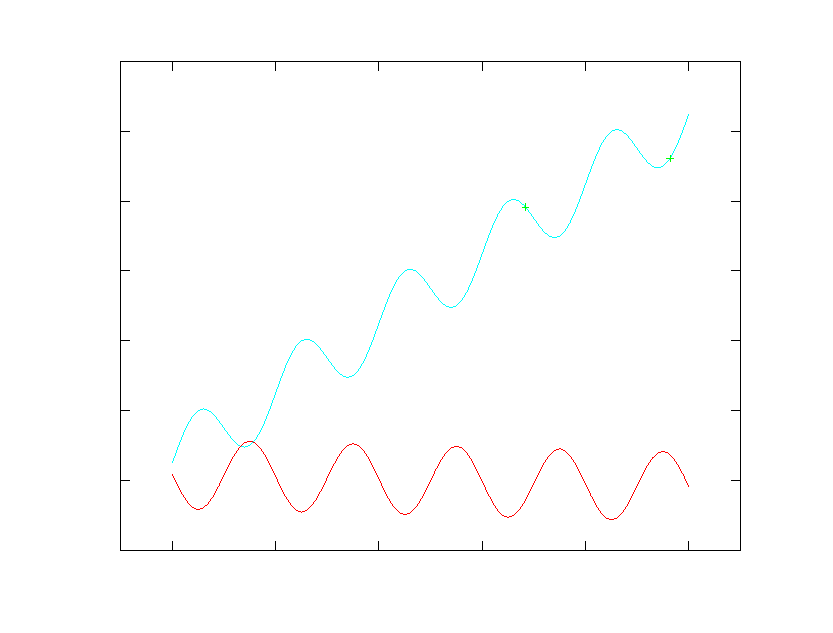
\includegraphics{SistemiLineari/exer332gamma10}}%
    \gplfronttext
  \end{picture}%
\endgroup

\end{center}
$gamma = 5e-1$: 
\begin{center}
% GNUPLOT: LaTeX picture with Postscript
\begingroup
  \makeatletter
  \providecommand\color[2][]{%
    \GenericError{(gnuplot) \space\space\space\@spaces}{%
      Package color not loaded in conjunction with
      terminal option `colourtext'%
    }{See the gnuplot documentation for explanation.%
    }{Either use 'blacktext' in gnuplot or load the package
      color.sty in LaTeX.}%
    \renewcommand\color[2][]{}%
  }%
  \providecommand\includegraphics[2][]{%
    \GenericError{(gnuplot) \space\space\space\@spaces}{%
      Package graphicx or graphics not loaded%
    }{See the gnuplot documentation for explanation.%
    }{The gnuplot epslatex terminal needs graphicx.sty or graphics.sty.}%
    \renewcommand\includegraphics[2][]{}%
  }%
  \providecommand\rotatebox[2]{#2}%
  \@ifundefined{ifGPcolor}{%
    \newif\ifGPcolor
    \GPcolortrue
  }{}%
  \@ifundefined{ifGPblacktext}{%
    \newif\ifGPblacktext
    \GPblacktexttrue
  }{}%
  % define a \g@addto@macro without @ in the name:
  \let\gplgaddtomacro\g@addto@macro
  % define empty templates for all commands taking text:
  \gdef\gplbacktext{}%
  \gdef\gplfronttext{}%
  \makeatother
  \ifGPblacktext
    % no textcolor at all
    \def\colorrgb#1{}%
    \def\colorgray#1{}%
  \else
    % gray or color?
    \ifGPcolor
      \def\colorrgb#1{\color[rgb]{#1}}%
      \def\colorgray#1{\color[gray]{#1}}%
      \expandafter\def\csname LTw\endcsname{\color{white}}%
      \expandafter\def\csname LTb\endcsname{\color{black}}%
      \expandafter\def\csname LTa\endcsname{\color{black}}%
      \expandafter\def\csname LT0\endcsname{\color[rgb]{1,0,0}}%
      \expandafter\def\csname LT1\endcsname{\color[rgb]{0,1,0}}%
      \expandafter\def\csname LT2\endcsname{\color[rgb]{0,0,1}}%
      \expandafter\def\csname LT3\endcsname{\color[rgb]{1,0,1}}%
      \expandafter\def\csname LT4\endcsname{\color[rgb]{0,1,1}}%
      \expandafter\def\csname LT5\endcsname{\color[rgb]{1,1,0}}%
      \expandafter\def\csname LT6\endcsname{\color[rgb]{0,0,0}}%
      \expandafter\def\csname LT7\endcsname{\color[rgb]{1,0.3,0}}%
      \expandafter\def\csname LT8\endcsname{\color[rgb]{0.5,0.5,0.5}}%
    \else
      % gray
      \def\colorrgb#1{\color{black}}%
      \def\colorgray#1{\color[gray]{#1}}%
      \expandafter\def\csname LTw\endcsname{\color{white}}%
      \expandafter\def\csname LTb\endcsname{\color{black}}%
      \expandafter\def\csname LTa\endcsname{\color{black}}%
      \expandafter\def\csname LT0\endcsname{\color{black}}%
      \expandafter\def\csname LT1\endcsname{\color{black}}%
      \expandafter\def\csname LT2\endcsname{\color{black}}%
      \expandafter\def\csname LT3\endcsname{\color{black}}%
      \expandafter\def\csname LT4\endcsname{\color{black}}%
      \expandafter\def\csname LT5\endcsname{\color{black}}%
      \expandafter\def\csname LT6\endcsname{\color{black}}%
      \expandafter\def\csname LT7\endcsname{\color{black}}%
      \expandafter\def\csname LT8\endcsname{\color{black}}%
    \fi
  \fi
  \setlength{\unitlength}{0.0500bp}%
  \begin{picture}(7680.00,5760.00)%
    \gplgaddtomacro\gplbacktext{%
      \colorrgb{0.00,0.00,0.00}%
      \put(866,634){\makebox(0,0)[r]{\strut{}-20}}%
      \colorrgb{0.00,0.00,0.00}%
      \put(866,1304){\makebox(0,0)[r]{\strut{}0}}%
      \colorrgb{0.00,0.00,0.00}%
      \put(866,1975){\makebox(0,0)[r]{\strut{}20}}%
      \colorrgb{0.00,0.00,0.00}%
      \put(866,2645){\makebox(0,0)[r]{\strut{}40}}%
      \colorrgb{0.00,0.00,0.00}%
      \put(866,3316){\makebox(0,0)[r]{\strut{}60}}%
      \colorrgb{0.00,0.00,0.00}%
      \put(866,3986){\makebox(0,0)[r]{\strut{}80}}%
      \colorrgb{0.00,0.00,0.00}%
      \put(866,4657){\makebox(0,0)[r]{\strut{}100}}%
      \colorrgb{0.00,0.00,0.00}%
      \put(866,5327){\makebox(0,0)[r]{\strut{}120}}%
      \colorrgb{0.00,0.00,0.00}%
      \put(1494,414){\makebox(0,0){\strut{}0}}%
      \colorrgb{0.00,0.00,0.00}%
      \put(2486,414){\makebox(0,0){\strut{}2}}%
      \colorrgb{0.00,0.00,0.00}%
      \put(3478,414){\makebox(0,0){\strut{}4}}%
      \colorrgb{0.00,0.00,0.00}%
      \put(4470,414){\makebox(0,0){\strut{}6}}%
      \colorrgb{0.00,0.00,0.00}%
      \put(5462,414){\makebox(0,0){\strut{}8}}%
      \colorrgb{0.00,0.00,0.00}%
      \put(6454,414){\makebox(0,0){\strut{}10}}%
    }%
    \gplgaddtomacro\gplfronttext{%
    }%
    \gplbacktext
    \put(0,0){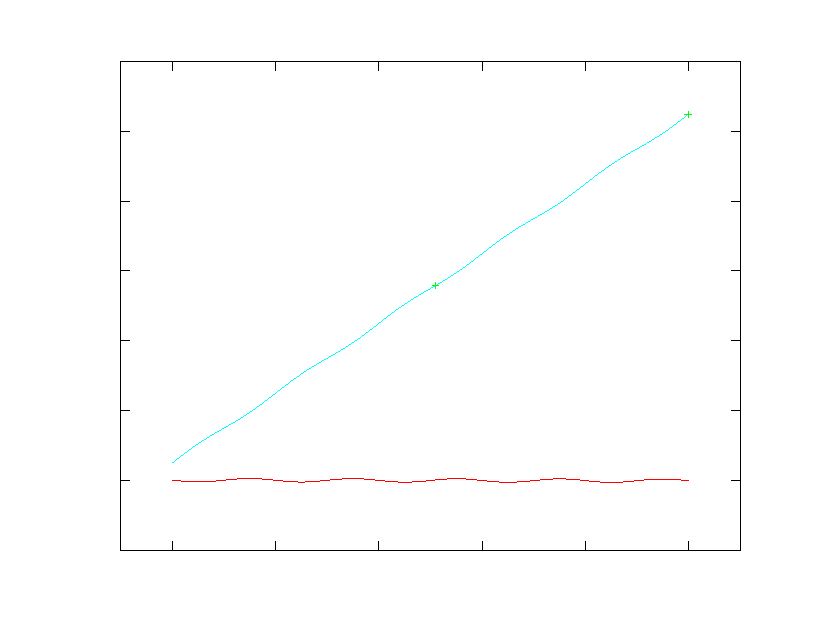
\includegraphics{SistemiLineari/exer332gamma5e-1}}%
    \gplfronttext
  \end{picture}%
\endgroup

\end{center}
$gamma = 1e-1$:
\begin{center}
% GNUPLOT: LaTeX picture with Postscript
\begingroup
  \makeatletter
  \providecommand\color[2][]{%
    \GenericError{(gnuplot) \space\space\space\@spaces}{%
      Package color not loaded in conjunction with
      terminal option `colourtext'%
    }{See the gnuplot documentation for explanation.%
    }{Either use 'blacktext' in gnuplot or load the package
      color.sty in LaTeX.}%
    \renewcommand\color[2][]{}%
  }%
  \providecommand\includegraphics[2][]{%
    \GenericError{(gnuplot) \space\space\space\@spaces}{%
      Package graphicx or graphics not loaded%
    }{See the gnuplot documentation for explanation.%
    }{The gnuplot epslatex terminal needs graphicx.sty or graphics.sty.}%
    \renewcommand\includegraphics[2][]{}%
  }%
  \providecommand\rotatebox[2]{#2}%
  \@ifundefined{ifGPcolor}{%
    \newif\ifGPcolor
    \GPcolortrue
  }{}%
  \@ifundefined{ifGPblacktext}{%
    \newif\ifGPblacktext
    \GPblacktexttrue
  }{}%
  % define a \g@addto@macro without @ in the name:
  \let\gplgaddtomacro\g@addto@macro
  % define empty templates for all commands taking text:
  \gdef\gplbacktext{}%
  \gdef\gplfronttext{}%
  \makeatother
  \ifGPblacktext
    % no textcolor at all
    \def\colorrgb#1{}%
    \def\colorgray#1{}%
  \else
    % gray or color?
    \ifGPcolor
      \def\colorrgb#1{\color[rgb]{#1}}%
      \def\colorgray#1{\color[gray]{#1}}%
      \expandafter\def\csname LTw\endcsname{\color{white}}%
      \expandafter\def\csname LTb\endcsname{\color{black}}%
      \expandafter\def\csname LTa\endcsname{\color{black}}%
      \expandafter\def\csname LT0\endcsname{\color[rgb]{1,0,0}}%
      \expandafter\def\csname LT1\endcsname{\color[rgb]{0,1,0}}%
      \expandafter\def\csname LT2\endcsname{\color[rgb]{0,0,1}}%
      \expandafter\def\csname LT3\endcsname{\color[rgb]{1,0,1}}%
      \expandafter\def\csname LT4\endcsname{\color[rgb]{0,1,1}}%
      \expandafter\def\csname LT5\endcsname{\color[rgb]{1,1,0}}%
      \expandafter\def\csname LT6\endcsname{\color[rgb]{0,0,0}}%
      \expandafter\def\csname LT7\endcsname{\color[rgb]{1,0.3,0}}%
      \expandafter\def\csname LT8\endcsname{\color[rgb]{0.5,0.5,0.5}}%
    \else
      % gray
      \def\colorrgb#1{\color{black}}%
      \def\colorgray#1{\color[gray]{#1}}%
      \expandafter\def\csname LTw\endcsname{\color{white}}%
      \expandafter\def\csname LTb\endcsname{\color{black}}%
      \expandafter\def\csname LTa\endcsname{\color{black}}%
      \expandafter\def\csname LT0\endcsname{\color{black}}%
      \expandafter\def\csname LT1\endcsname{\color{black}}%
      \expandafter\def\csname LT2\endcsname{\color{black}}%
      \expandafter\def\csname LT3\endcsname{\color{black}}%
      \expandafter\def\csname LT4\endcsname{\color{black}}%
      \expandafter\def\csname LT5\endcsname{\color{black}}%
      \expandafter\def\csname LT6\endcsname{\color{black}}%
      \expandafter\def\csname LT7\endcsname{\color{black}}%
      \expandafter\def\csname LT8\endcsname{\color{black}}%
    \fi
  \fi
  \setlength{\unitlength}{0.0500bp}%
  \begin{picture}(7680.00,5760.00)%
    \gplgaddtomacro\gplbacktext{%
      \colorrgb{0.00,0.00,0.00}%
      \put(866,634){\makebox(0,0)[r]{\strut{}-20}}%
      \colorrgb{0.00,0.00,0.00}%
      \put(866,1304){\makebox(0,0)[r]{\strut{}0}}%
      \colorrgb{0.00,0.00,0.00}%
      \put(866,1975){\makebox(0,0)[r]{\strut{}20}}%
      \colorrgb{0.00,0.00,0.00}%
      \put(866,2645){\makebox(0,0)[r]{\strut{}40}}%
      \colorrgb{0.00,0.00,0.00}%
      \put(866,3316){\makebox(0,0)[r]{\strut{}60}}%
      \colorrgb{0.00,0.00,0.00}%
      \put(866,3986){\makebox(0,0)[r]{\strut{}80}}%
      \colorrgb{0.00,0.00,0.00}%
      \put(866,4657){\makebox(0,0)[r]{\strut{}100}}%
      \colorrgb{0.00,0.00,0.00}%
      \put(866,5327){\makebox(0,0)[r]{\strut{}120}}%
      \colorrgb{0.00,0.00,0.00}%
      \put(1494,414){\makebox(0,0){\strut{}0}}%
      \colorrgb{0.00,0.00,0.00}%
      \put(2486,414){\makebox(0,0){\strut{}2}}%
      \colorrgb{0.00,0.00,0.00}%
      \put(3478,414){\makebox(0,0){\strut{}4}}%
      \colorrgb{0.00,0.00,0.00}%
      \put(4470,414){\makebox(0,0){\strut{}6}}%
      \colorrgb{0.00,0.00,0.00}%
      \put(5462,414){\makebox(0,0){\strut{}8}}%
      \colorrgb{0.00,0.00,0.00}%
      \put(6454,414){\makebox(0,0){\strut{}10}}%
    }%
    \gplgaddtomacro\gplfronttext{%
    }%
    \gplbacktext
    \put(0,0){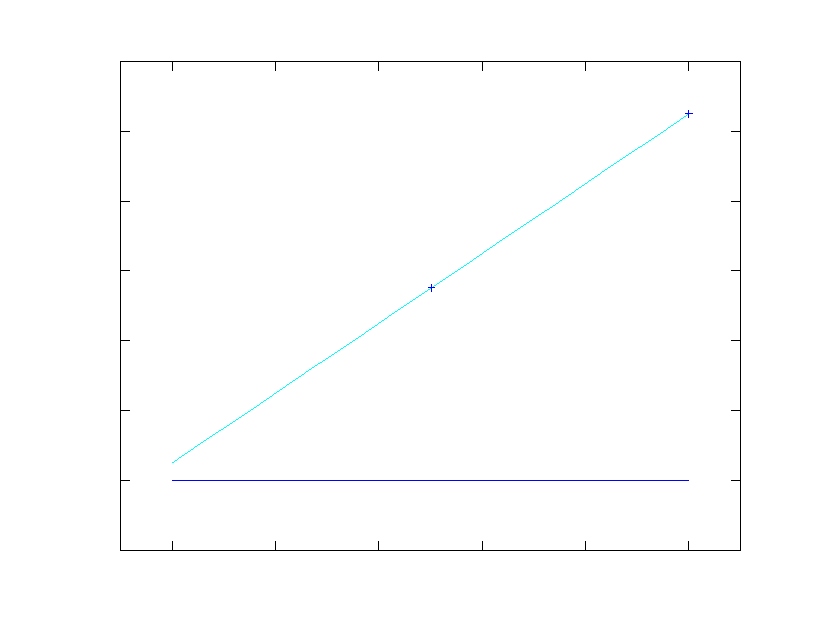
\includegraphics{SistemiLineari/exer332gammae-1}}%
    \gplfronttext
  \end{picture}%
\endgroup

\end{center}
$gamma = 1e-3$:
\begin{center}
% GNUPLOT: LaTeX picture with Postscript
\begingroup
  \makeatletter
  \providecommand\color[2][]{%
    \GenericError{(gnuplot) \space\space\space\@spaces}{%
      Package color not loaded in conjunction with
      terminal option `colourtext'%
    }{See the gnuplot documentation for explanation.%
    }{Either use 'blacktext' in gnuplot or load the package
      color.sty in LaTeX.}%
    \renewcommand\color[2][]{}%
  }%
  \providecommand\includegraphics[2][]{%
    \GenericError{(gnuplot) \space\space\space\@spaces}{%
      Package graphicx or graphics not loaded%
    }{See the gnuplot documentation for explanation.%
    }{The gnuplot epslatex terminal needs graphicx.sty or graphics.sty.}%
    \renewcommand\includegraphics[2][]{}%
  }%
  \providecommand\rotatebox[2]{#2}%
  \@ifundefined{ifGPcolor}{%
    \newif\ifGPcolor
    \GPcolortrue
  }{}%
  \@ifundefined{ifGPblacktext}{%
    \newif\ifGPblacktext
    \GPblacktexttrue
  }{}%
  % define a \g@addto@macro without @ in the name:
  \let\gplgaddtomacro\g@addto@macro
  % define empty templates for all commands taking text:
  \gdef\gplbacktext{}%
  \gdef\gplfronttext{}%
  \makeatother
  \ifGPblacktext
    % no textcolor at all
    \def\colorrgb#1{}%
    \def\colorgray#1{}%
  \else
    % gray or color?
    \ifGPcolor
      \def\colorrgb#1{\color[rgb]{#1}}%
      \def\colorgray#1{\color[gray]{#1}}%
      \expandafter\def\csname LTw\endcsname{\color{white}}%
      \expandafter\def\csname LTb\endcsname{\color{black}}%
      \expandafter\def\csname LTa\endcsname{\color{black}}%
      \expandafter\def\csname LT0\endcsname{\color[rgb]{1,0,0}}%
      \expandafter\def\csname LT1\endcsname{\color[rgb]{0,1,0}}%
      \expandafter\def\csname LT2\endcsname{\color[rgb]{0,0,1}}%
      \expandafter\def\csname LT3\endcsname{\color[rgb]{1,0,1}}%
      \expandafter\def\csname LT4\endcsname{\color[rgb]{0,1,1}}%
      \expandafter\def\csname LT5\endcsname{\color[rgb]{1,1,0}}%
      \expandafter\def\csname LT6\endcsname{\color[rgb]{0,0,0}}%
      \expandafter\def\csname LT7\endcsname{\color[rgb]{1,0.3,0}}%
      \expandafter\def\csname LT8\endcsname{\color[rgb]{0.5,0.5,0.5}}%
    \else
      % gray
      \def\colorrgb#1{\color{black}}%
      \def\colorgray#1{\color[gray]{#1}}%
      \expandafter\def\csname LTw\endcsname{\color{white}}%
      \expandafter\def\csname LTb\endcsname{\color{black}}%
      \expandafter\def\csname LTa\endcsname{\color{black}}%
      \expandafter\def\csname LT0\endcsname{\color{black}}%
      \expandafter\def\csname LT1\endcsname{\color{black}}%
      \expandafter\def\csname LT2\endcsname{\color{black}}%
      \expandafter\def\csname LT3\endcsname{\color{black}}%
      \expandafter\def\csname LT4\endcsname{\color{black}}%
      \expandafter\def\csname LT5\endcsname{\color{black}}%
      \expandafter\def\csname LT6\endcsname{\color{black}}%
      \expandafter\def\csname LT7\endcsname{\color{black}}%
      \expandafter\def\csname LT8\endcsname{\color{black}}%
    \fi
  \fi
  \setlength{\unitlength}{0.0500bp}%
  \begin{picture}(7680.00,5760.00)%
    \gplgaddtomacro\gplbacktext{%
      \colorrgb{0.00,0.00,0.00}%
      \put(866,634){\makebox(0,0)[r]{\strut{}-20}}%
      \colorrgb{0.00,0.00,0.00}%
      \put(866,1304){\makebox(0,0)[r]{\strut{}0}}%
      \colorrgb{0.00,0.00,0.00}%
      \put(866,1975){\makebox(0,0)[r]{\strut{}20}}%
      \colorrgb{0.00,0.00,0.00}%
      \put(866,2645){\makebox(0,0)[r]{\strut{}40}}%
      \colorrgb{0.00,0.00,0.00}%
      \put(866,3316){\makebox(0,0)[r]{\strut{}60}}%
      \colorrgb{0.00,0.00,0.00}%
      \put(866,3986){\makebox(0,0)[r]{\strut{}80}}%
      \colorrgb{0.00,0.00,0.00}%
      \put(866,4657){\makebox(0,0)[r]{\strut{}100}}%
      \colorrgb{0.00,0.00,0.00}%
      \put(866,5327){\makebox(0,0)[r]{\strut{}120}}%
      \colorrgb{0.00,0.00,0.00}%
      \put(1494,414){\makebox(0,0){\strut{}0}}%
      \colorrgb{0.00,0.00,0.00}%
      \put(2486,414){\makebox(0,0){\strut{}2}}%
      \colorrgb{0.00,0.00,0.00}%
      \put(3478,414){\makebox(0,0){\strut{}4}}%
      \colorrgb{0.00,0.00,0.00}%
      \put(4470,414){\makebox(0,0){\strut{}6}}%
      \colorrgb{0.00,0.00,0.00}%
      \put(5462,414){\makebox(0,0){\strut{}8}}%
      \colorrgb{0.00,0.00,0.00}%
      \put(6454,414){\makebox(0,0){\strut{}10}}%
    }%
    \gplgaddtomacro\gplfronttext{%
    }%
    \gplbacktext
    \put(0,0){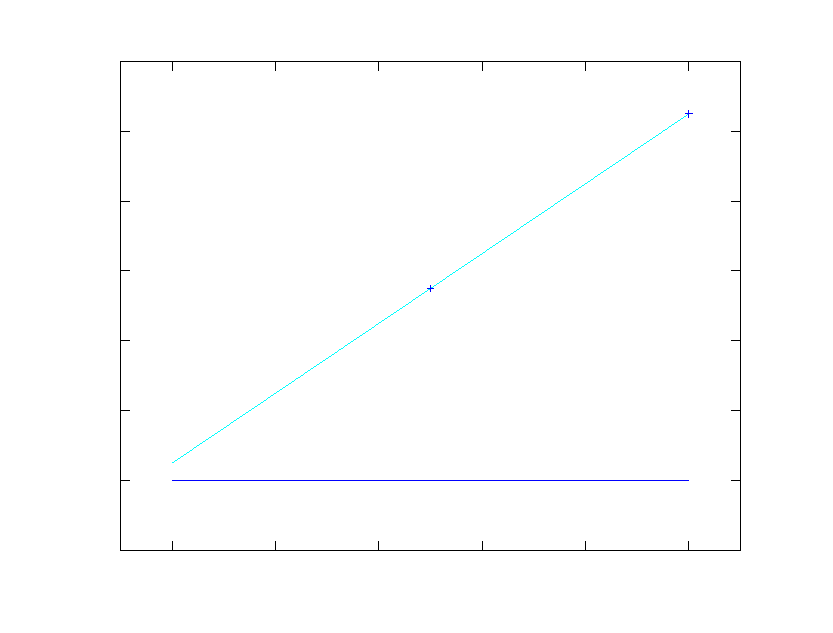
\includegraphics{SistemiLineari/exer332gammae-3}}%
    \gplfronttext
  \end{picture}%
\endgroup

\end{center}
Per $gamma \rightarrow \infty$ si raggiunge la soluzione ottima del sistema
$A\vect{x} = \vect{b} + \vect{r}$ con $\vect{r} = \vect{0}$.
